% Ask the Sensors -- CS60055 Hackathon Challenge 1 technical report.
% Build: cd docs/report && pdflatex report.tex && pdflatex report.tex
% Every number below comes from a committed file under results/ or models/;
% the repository README lists the command that regenerates each one.
\documentclass[11pt,a4paper]{article}
\usepackage[margin=2.1cm]{geometry}
\usepackage{amsmath}
\usepackage{lmodern}
\usepackage[T1]{fontenc}
\usepackage{microtype}
\usepackage{graphicx}
\usepackage{booktabs}
\usepackage{caption}
\usepackage{xcolor}
\usepackage{enumitem}
\usepackage{tikz}
\usetikzlibrary{positioning,arrows.meta,decorations.pathreplacing}
\usepackage[hidelinks]{hyperref}
\graphicspath{{../../results/}}
\setlist{nosep,leftmargin=1.4em}
\captionsetup{font=small,labelfont=bf}
% Explanatory diagrams get their own numbering, so the five result figures
% keep the numbers printed inside their images.
\DeclareCaptionType{diagram}[Diagram][List of Diagrams]
\setlength{\parskip}{0.35em}
\newcommand{\code}[1]{\texttt{#1}}

\title{\textbf{Ask the Sensors}\\[2pt]\large Answering questions about daily activity from motion sensors, with evidence}
\author{Abhinav Kumar Singh (22CS30005) \qquad Harsh Chattar (22CS30028)\\
\small CS60055 Ubiquitous Computing, IIT Kharagpur --- Hackathon Challenge 1\\
\small \url{https://github.com/code-Harsh247/AskTheSensors}}
\date{}

\begin{document}
\maketitle

\begin{abstract}
\noindent Our system answers plain-language questions about a person's activity, such as ``how long was she walking?'', from a phone's accelerometer and gyroscope, and shows the stretch of signal each answer is based on. A small neural network labels the recording; ordinary code then computes every answer and its evidence, and a checker blocks any answer whose evidence does not hold up. Given correct activity labels, the system answers all 87 of our test questions correctly. With the trained model it answers 15 of 34 on real users, and all 19 misses trace back to recognition errors, not to the question answering.
\end{abstract}

% ---------------------------------------------------------------------
\section{Introduction}
The challenge describes an older woman living alone, whose son and physiotherapist want to ask about her day and trust the answers, without cameras. An activity classifier alone says what she is doing at each moment, but not for how long, how often, when, or why. So every answer here must come with evidence. Three ideas shaped our design:
\begin{enumerate}
  \item \textbf{Numbers come from code, not from a language model,} so they can be checked.
  \item \textbf{``I can't tell'' beats a confident wrong answer.} Without enough evidence, the system answers \code{N/A} and says why.
  \item \textbf{Keep recognition and reasoning separable.} Answering every question from both the true labels and the model's labels shows which part caused each mistake.
\end{enumerate}
Every number in this report can be regenerated with the commands in the repository README.

% ---------------------------------------------------------------------
\section{How it works}
The system has two halves, built separately and joined by one agreed file (Diagram~\ref{dg:overview}). The first half turns the raw recording into a label for every 4-second window. The second half builds a timeline from those labels and uses it to answer questions. Because the file format was fixed first, the answering half was built and tested on true labels long before the model existed.

\begin{diagram}[h]
\centering
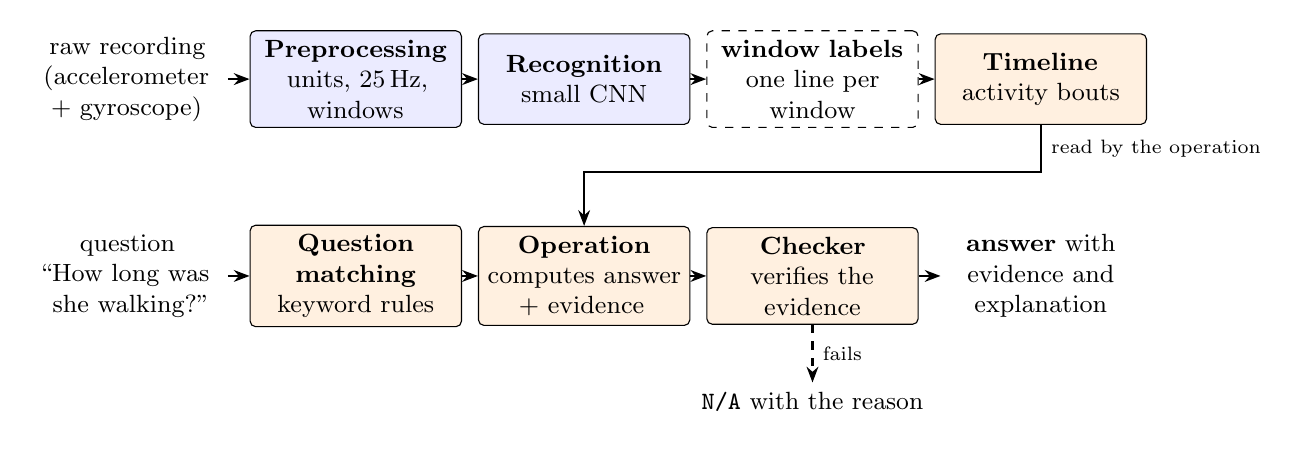
\begin{tikzpicture}[
  sig/.style={draw, rounded corners=2pt, fill=blue!8, align=center, font=\small, minimum height=1.15cm, text width=2.45cm},
  ans/.style={draw, rounded corners=2pt, fill=orange!12, align=center, font=\small, minimum height=1.15cm, text width=2.45cm},
  io/.style={align=center, font=\small, text width=2.3cm},
  arr/.style={-{Stealth[length=2mm]}, thick}]
\node[io]  (rec)  at (0,0)    {raw recording\\(accelerometer + gyroscope)};
\node[sig] (pre)  at (2.9,0)  {\textbf{Preprocessing}\\units, 25\,Hz, windows};
\node[sig] (cnn)  at (5.8,0)  {\textbf{Recognition}\\small CNN};
\node[draw, dashed, rounded corners=2pt, align=center, font=\small, minimum height=1.15cm, text width=2.45cm] (file) at (8.7,0) {\textbf{window labels}\\one line per window};
\node[ans] (tl)   at (11.6,0) {\textbf{Timeline}\\activity bouts};
\node[io]  (q)    at (0,-2.5)   {question\\``How long was she walking?''};
\node[ans] (rt)   at (2.9,-2.5) {\textbf{Question matching}\\keyword rules};
\node[ans] (op)   at (5.8,-2.5) {\textbf{Operation}\\computes answer + evidence};
\node[ans] (chk)  at (8.7,-2.5) {\textbf{Checker}\\verifies the evidence};
\node[io]  (out)  at (11.6,-2.5) {\textbf{answer} with evidence and explanation};
\node[font=\small] (na) at (8.7,-4.1) {\code{N/A} with the reason};
\draw[arr] (rec) -- (pre); \draw[arr] (pre) -- (cnn); \draw[arr] (cnn) -- (file); \draw[arr] (file) -- (tl);
\draw[arr] (q) -- (rt); \draw[arr] (rt) -- (op); \draw[arr] (op) -- (chk); \draw[arr] (chk) -- (out);
\draw[arr] (tl.south) -- node[right, font=\scriptsize]{read by the operation} ++(0,-0.6) -| (op.north);
\draw[arr, dashed] (chk) -- node[right, font=\scriptsize]{fails} (na);
\end{tikzpicture}
\caption{The whole system. Blue parts were built by Abhinav, orange parts by Harsh; the dashed box is the file that joins them.}
\label{dg:overview}
\end{diagram}

\subsection{Data and preprocessing}
We use the ExtraSensory dataset~\cite{extrasensory}: 60 people recorded during ordinary life. From each we take the phone's accelerometer and gyroscope, three axes each, and the activity the person reported. The phone does not record continuously. It captures a burst of about 20 seconds in every minute, at an uneven rate of around 40 samples per second, and the person's label covers that whole minute (Diagram~\ref{dg:minute}).

Before anything else, the raw signal is cleaned in three steps:
\begin{enumerate}
  \item \textbf{Units.} Some phones record acceleration in $g$, others in m/s$^2$. Using one conversion for everyone left one person apparently experiencing ten times gravity while at rest. We now decide the unit per person, by checking whether their typical reading is close to 1 or to 9.8. This fixed 59 of the 60 people; the one that fits neither is flagged.
  \item \textbf{Resampling.} Every signal is resampled onto an exact 25\,Hz grid, so all recordings share one time base. Stretches with no real samples are marked as missing instead of being filled in with invented values.
  \item \textbf{Windows.} The signal is cut into 4-second windows, starting a new one every 2 seconds, so neighbouring windows overlap by half. A window is 101 samples on each of the 6 channels. Each window also records how much of it was really recorded, and a short summary of the signal: how strong and how variable the acceleration is, how much the gyroscope turns, and the rhythm of any repeating motion such as steps. The answering half quotes this summary in its explanations.
\end{enumerate}

\begin{diagram}[h]
\centering
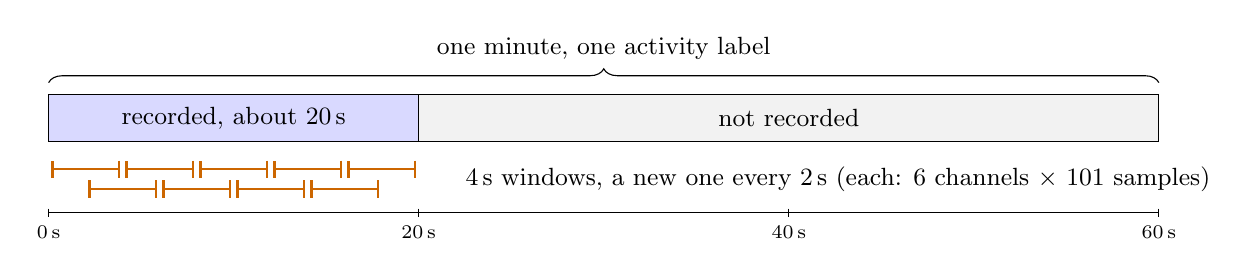
\begin{tikzpicture}[x=0.235cm, y=1cm]
\draw[fill=blue!15] (0,0) rectangle (20,0.6) node[midway, font=\small] {recorded, about 20\,s};
\draw[fill=gray!10] (20,0) rectangle (60,0.6) node[midway, font=\small] {not recorded};
\draw[decorate, decoration={brace, amplitude=5pt}] (0,0.75) -- (60,0.75) node[midway, above=5pt, font=\small] {one minute, one activity label};
\foreach \k in {0,...,8} {
  \pgfmathsetmacro{\y}{-0.35-0.25*mod(\k,2)}
  \draw[thick, orange!80!black, |-|] (2*\k+0.15,\y) -- (2*\k+3.85,\y);
}
\node[font=\small, anchor=west] at (22,-0.48) {4\,s windows, a new one every 2\,s (each: 6 channels $\times$ 101 samples)};
\foreach \t in {0,20,40,60} { \draw (\t,-0.85) -- (\t,-0.95) node[below, font=\scriptsize] {\t\,s}; }
\draw (0,-0.9) -- (60,-0.9);
\end{tikzpicture}
\caption{One recorded minute. Only the first 20 seconds or so hold signal; the windows are cut from that burst.}
\label{dg:minute}
\end{diagram}

\subsection{Recognising the activity in each window}
A small convolutional neural network, built with PyTorch~\cite{torch}, reads each window and outputs a probability for each of the seven activities (Diagram~\ref{dg:cnn}). Its three convolution layers learn short motion patterns across the six channels, such as the rhythm of steps or the stillness of lying. Two pooling steps halve the length of the signal along the way. Averaging over time then gives a single summary of the window, and a final layer turns it into the seven probabilities.

The network has only 9,975 parameters (48\,KB), small enough to run on a phone and easy to compress further (Section~\ref{sec:efficiency}). It was trained on 36 people and checked on 12 others, so no person's data is used for both. Because some activities are rare (running is 0.6\% of the training windows), rare activities are weighted up during training.

\begin{diagram}[h]
\centering
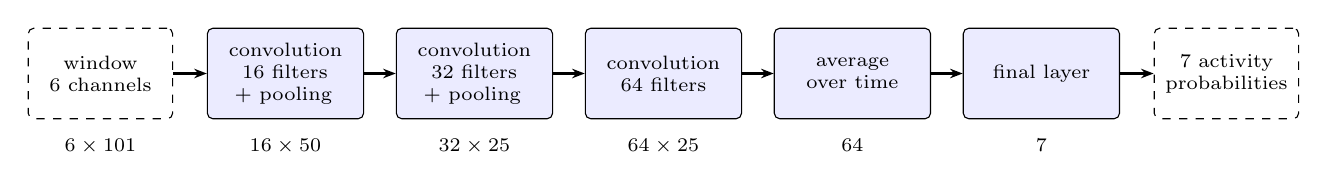
\begin{tikzpicture}[
  layer/.style={draw, rounded corners=2pt, fill=blue!8, align=center, font=\scriptsize, minimum height=1.15cm, text width=1.75cm},
  dims/.style={font=\scriptsize\itshape, align=center},
  arr/.style={-{Stealth[length=1.6mm]}, thick}]
\node[draw, dashed, rounded corners=2pt, align=center, font=\scriptsize, minimum height=1.15cm, text width=1.6cm] (in) at (0,0) {window\\6 channels};
\node[layer] (c1) at (2.35,0)  {convolution\\16 filters\\+ pooling};
\node[layer] (c2) at (4.75,0)  {convolution\\32 filters\\+ pooling};
\node[layer] (c3) at (7.15,0)  {convolution\\64 filters};
\node[layer] (gp) at (9.55,0)  {average\\over time};
\node[layer] (fc) at (11.95,0) {final layer};
\node[draw, dashed, rounded corners=2pt, align=center, font=\scriptsize, minimum height=1.15cm, text width=1.6cm] (out) at (14.3,0) {7 activity\\probabilities};
\foreach \a/\b in {in/c1, c1/c2, c2/c3, c3/gp, gp/fc, fc/out} { \draw[arr] (\a) -- (\b); }
\node[dims, below=0.12cm of in] {$6 \times 101$};
\node[dims, below=0.12cm of c1] {$16 \times 50$};
\node[dims, below=0.12cm of c2] {$32 \times 25$};
\node[dims, below=0.12cm of c3] {$64 \times 25$};
\node[dims, below=0.12cm of gp] {$64$};
\node[dims, below=0.12cm of fc] {$7$};
\end{tikzpicture}
\caption{The recognition network. The numbers underneath give the size of the data after each step (channels $\times$ time steps).}
\label{dg:cnn}
\end{diagram}

For each window the recognition half writes one line to the shared file: the seven probabilities, how much of the window was really recorded, and the signal summary.

\subsection{Building a timeline}
Questions are about bouts of activity (``how long'', ``how many times''), not about windows. Adding up windows would also give the wrong answer, because the phone records only about a third of each minute: a 30-minute walk would come out as roughly 10 minutes. So the timeline is built minute by minute (Diagram~\ref{dg:timeline}):
\begin{itemize}
  \item all windows in a burst are given one shared label, the activity with the highest total probability, so a single misread window cannot create a fake bout;
  \item each burst then stands for its whole minute, and neighbouring minutes with the same activity join into one bout;
  \item a minute with no recording stays a gap, so the system never claims to know what happened when nothing was recorded;
  \item gaps shorter than a minute, caused by the phone's clock drifting, are closed, because they cannot hide a whole missing minute. On one person this turned 3,151 broken-up bouts into 325 real ones.
\end{itemize}

\begin{diagram}[h]
\centering
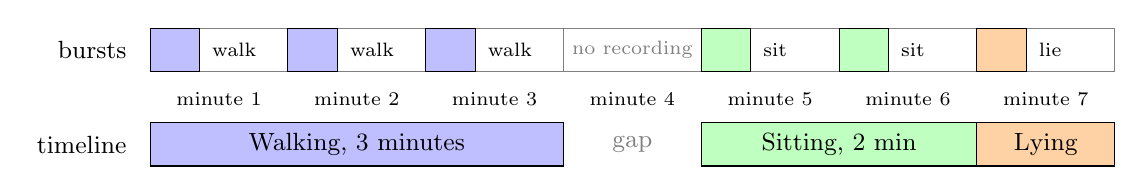
\begin{tikzpicture}[x=1.75cm, y=1cm]
\foreach \i in {0,...,6} { \draw[gray] (\i,1.2) rectangle ++(1,0.55); \node[font=\scriptsize] at (\i+0.5,0.85) {minute \the\numexpr\i+1\relax}; }
\foreach \i/\lab/\col in {0/walk/blue!25, 1/walk/blue!25, 2/walk/blue!25, 4/sit/green!25, 5/sit/green!25, 6/lie/orange!35} {
  \draw[fill=\col] (\i,1.2) rectangle ++(0.36,0.55); \node[font=\scriptsize, anchor=west] at (\i+0.38,1.475) {\lab};
}
\node[font=\scriptsize, text=gray] at (3.5,1.475) {no recording};
\draw[fill=blue!25] (0,0) rectangle (3,0.55) node[midway, font=\small] {Walking, 3 minutes};
\node[font=\small, text=gray] at (3.5,0.275) {gap};
\draw[fill=green!25] (4,0) rectangle (6,0.55) node[midway, font=\small] {Sitting, 2 min};
\draw[fill=orange!35] (6,0) rectangle (7,0.55) node[midway, font=\small] {Lying};
\node[font=\small, anchor=east] at (-0.1,1.475) {bursts};
\node[font=\small, anchor=east] at (-0.1,0.275) {timeline};
\end{tikzpicture}
\caption{From bursts to bouts. Each short coloured block is a recorded burst with its shared label. Each burst stands for its minute, same-activity minutes join into bouts, and the unrecorded minute stays a gap.}
\label{dg:timeline}
\end{diagram}

\subsection{Answering a question}
Each question goes through three steps, left to right along the bottom row of Diagram~\ref{dg:overview}.

\textbf{Matching the question.} Keyword rules pick out the activity named (``walking'', ``jogging'', ``lying down''), any time mentioned (``at 340 seconds''), and words that signal the kind of question (``how long'', ``how many times'', ``when did she start''). Together these choose one of eight operations (Table~\ref{tab:ops}). We also tried a small language model, Qwen2.5-0.5B~\cite{qwen}, for this step, allowed only to choose the operation, never to produce the answer. It did worse: on 13 new questions it matched 46\% correctly against 69\% for the rules, and it took 11.4\,s per question against 67\,ms. So the rules are the default.

\begin{table}[h]
\centering\small
\begin{tabular}{@{}lll@{}}
\toprule
Operation & Example question & What it returns \\
\midrule
Identify & What was the user doing at 340 seconds? & the activity, and its interval \\
Verify & Is the user running? & yes or no, and where \\
Duration & How long was the user walking? & total time, and every walking interval \\
Count & How many times did the user walk? & number of bouts, and the bouts \\
Compare & More time walking or running? & the longer one, and both totals \\
Find start & Did the user begin running, and when? & the start time, and the first bout \\
Show evidence & Cite the evidence for walking. & the intervals \\
Open-ended & Was the user resting for a long time? & a verdict argued from the signal \\
\bottomrule
\end{tabular}
\caption{The eight operations.}
\label{tab:ops}
\end{table}

\textbf{Computing the answer.} The chosen operation reads the timeline and calculates the answer in ordinary code: adding up bout lengths, counting bouts, or finding the first one. It also collects the intervals the answer rests on, and writes an explanation that quotes the measured signal summary for those intervals. A ``no'' answer is backed by evidence too: ``did she run?'' answered ``no'' lists every interval that was checked. Here is a real answer from a 46-hour recording, with the list of intervals shortened:
{\small
\begin{verbatim}
Query: "Was the user resting for a long time?"
Answer:              Likely yes
Activity/Event:      Sustained stillness
Evidence:
    Timestamp(s):        5758 to 6548, 7579 to 8249, ...
    Sensor Modality:     Accelerometer, Gyroscope
    Sensor Channel(s):   All
Explanation:         The longest stretch of mostly still signal runs 216560-237464 s
                     (20904 s), at or above the 300 s taken as prolonged; ...
\end{verbatim}}

\textbf{Questions beyond the seven activities.} Some questions ask about things the model was never trained to name, such as ``was she resting for a long time?'', ``was she fidgeting?'' or ``did she take a nap?''. For these the system does not rely on the labels. It measures how \emph{still} the signal is. A window counts as still when its acceleration barely varies (a standard deviation of at most 0.022\,m/s$^2$) and the gyroscope barely turns. These limits were set from the lying-down windows of one person. On a second person, 97\% of lying windows count as still, and none of the walking, running or cycling windows do. This one measurement supports several answers:
\begin{itemize}
  \item \textbf{long rest:} the longest run of still minutes, whether the model called it sitting or lying;
  \item \textbf{sleep:} the same evidence, with the explanation stating that motion sensors cannot tell sleep from lying awake;
  \item \textbf{restlessness:} movement while the person is seated or lying;
  \item \textbf{a veto on claims like ``cycling'' or ``strenuous''} when the signal is actually still.
\end{itemize}
For behaviours we have no measurement for, such as driving or climbing stairs, the system answers that it cannot tell, rather than guessing the closest of the seven activities.

\subsection{Checking every answer}
Before any answer is released, a checker tests it against the timeline:
\begin{itemize}
  \item every interval it cites must really exist in the timeline;
  \item the times written in the answer must match the cited intervals;
  \item a question that needs evidence must have some;
  \item every duration and count must add up again from the cited intervals.
\end{itemize}
If any check fails, the answer is withheld and replaced by \code{N/A} with the reason (the dashed arrow in Diagram~\ref{dg:overview}). This makes an unsupported answer impossible by construction, rather than merely unlikely. In all our test runs the checker never had to step in.

% ---------------------------------------------------------------------
\section{How we evaluated}
\label{sec:eval}

\paragraph{Test questions.} We wrote two sets of questions covering every kind of question the challenge describes, each stored with its correct answer:
\begin{itemize}
  \item \textbf{53 questions about three simulated users,} whose recordings follow the same minute-by-minute pattern as the real data. Because we generated their schedules, we know the true answers exactly. The set includes deliberately awkward cases: an activity that never happens, a question about a moment with no recording, and two activities that took exactly as long.
  \item \textbf{34 questions about two real users} from the dataset. Their correct answers were computed from the users' own activity labels by a separate piece of code, written independently of the system's timeline code. The two had to agree exactly before any answer was saved, and they did.
\end{itemize}

\paragraph{When is an answer correct?} Different kinds of answer need different rules (Table~\ref{tab:rules}). For evidence, we measure how much the cited interval overlaps the true one: the shared time divided by the combined time. It must be at least 50\%, meaning the cited interval covers more of the truth than it misses. The 4-second tolerance on durations is two window steps, the finest a boundary can be placed; the 10\% part stops long bouts from having to be exact to the second. All thresholds were fixed before we saw any results, so they could not be tuned to flatter the scores. Figure~\ref{fig:fig3} shows how the scores change if they are made looser or stricter. The overall score averages the seven question types equally, so plentiful easy questions cannot dominate it.

\begin{table}[h]
\centering\small
\begin{tabular}{@{}ll@{}}
\toprule
Question type & Counted correct when \\
\midrule
Identification & it names the right activity \\
Verification & the yes/no answer is right \\
Duration & it is within 4\,s or 10\% of the true total, whichever is larger \\
Count & it is within 1 of the true number of bouts \\
Comparison & it names the activity that took longer (or ``equal'', within 2\,s) \\
Grounding & the cited intervals overlap the true ones by at least 50\% \\
Open-world & the verdict matches the expected one \\
\bottomrule
\end{tabular}
\caption{The rule for a correct answer, per question type.}
\label{tab:rules}
\end{table}

\paragraph{Finding which part made a mistake.} Every question is answered twice by exactly the same answering code: once from the true activity labels, and once from the labels the model predicted (Diagram~\ref{dg:eval}). Comparing the two answers with the correct one shows where each mistake came from.

\begin{diagram}[h]
\centering
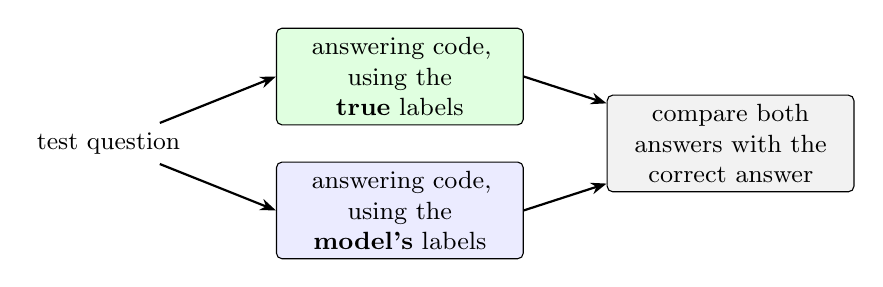
\begin{tikzpicture}[
  box/.style={draw, rounded corners=2pt, align=center, font=\small, minimum height=1.0cm, text width=2.9cm},
  arr/.style={-{Stealth[length=2mm]}, thick}]
\node[align=center, font=\small] (q) at (0,0) {test question};
\node[box, fill=green!12] (t) at (3.7,0.85) {answering code,\\using the \textbf{true} labels};
\node[box, fill=blue!8] (m) at (3.7,-0.85) {answering code,\\using the \textbf{model's} labels};
\node[box, fill=gray!10] (c) at (7.9,0) {compare both answers with the correct answer};
\draw[arr] (q) -- (t.west); \draw[arr] (q) -- (m.west);
\draw[arr] (t.east) -- (c); \draw[arr] (m.east) -- (c);
\end{tikzpicture}
\par\medskip
{\small
\begin{tabular}{@{}lll@{}}
\toprule
With true labels & With the model's labels & Meaning \\
\midrule
right & right & correct \\
right & wrong & recognition error \\
wrong & either & answering error \\
\bottomrule
\end{tabular}}
\caption{How each mistake is traced. The answering code is identical on both paths, so if it is right with true labels but wrong with the model's, the mistake must come from recognition.}
\label{dg:eval}
\end{diagram}

\paragraph{Stress test.} To see how the answering copes with recognition mistakes of a known size, we deliberately mislabelled a random 10\% of the recorded minutes of the simulated users and answered all 53 questions again.

\paragraph{Open-ended questions and explanations.} We asked 16 more questions about behaviours outside the seven activities, such as fidgeting or driving, to check that each is either argued from the signal or honestly declined. Explanations cannot be scored by exact match, so a separate language model, Claude Haiku 4.5~\cite{claude}, rated each open-ended explanation from 1 to 5 on three questions: does it cite real signal measurements, do they support the answer, and is the answer plausible. It was shown the values the system actually measured, so it could catch a number that did not match the signal. It rated every explanation twice, independently, and the agreement between the two runs (weighted $\kappa$) tells us how consistent it is.

% ---------------------------------------------------------------------
\section{Results}

\paragraph{Answering questions.} Given true labels, the system answers every question correctly: all 53 simulated and all 34 real. In the stress test, with 10\% of the minutes mislabelled, the overall score fell only to 84\% and correct evidence to 69\%. Durations were hit hardest (56\%), because one wrong minute moves a total by a whole minute. With the trained model's labels it gets 15 of the 34 real-user questions (39\% averaged over question types), and all 19 misses are recognition errors (Figure~\ref{fig:fig1}). Durations, counts and comparisons fail completely, because they add up the model's mistakes over tens of hours; on one user it reports 42 bouts of an activity that really has 5. Yes/no and open-ended questions hold up best.

\begin{figure}[h]
\centering
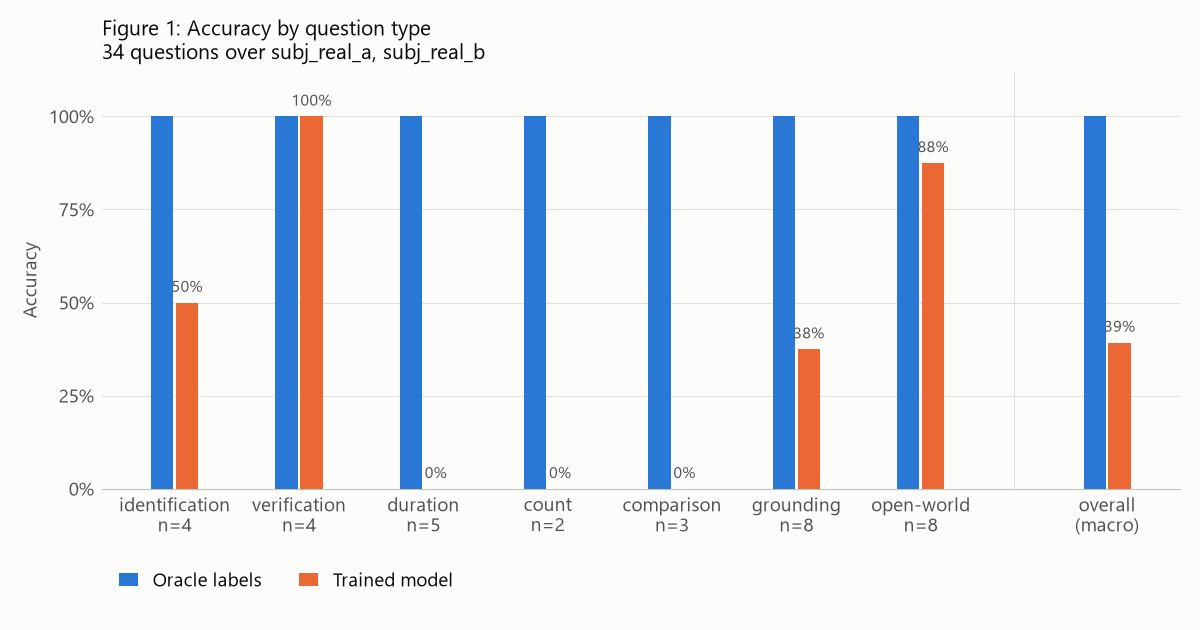
\includegraphics[width=0.78\linewidth]{fig1_accuracy_by_question_type.png}
\caption{\textbf{Accuracy by question type} on 34 real-user questions, from true labels (blue) and the model's labels (orange). Correct means: identification, the right activity; verification, the right yes/no; duration, within 4\,s or 10\%; count, within 1; comparison, the activity that took longer; grounding, cited evidence overlapping the truth by at least 50\%; open-world, the expected verdict. ``Overall'' averages the types equally.}
\label{fig:fig1}
\end{figure}

\paragraph{Recognition.} On held-out users the model reaches a macro-F1 of 0.289, against 0.079 for always guessing the most common activity and 0.225 for logistic regression (Figure~\ref{fig:fig2}). Its biggest error is mistaking sitting for lying (43.8\% of sitting windows); both are still postures that differ mainly in the phone's angle. It almost never recognises ``standing in place'', which has no distinctive signal, or running, which is rare in the data.

\begin{figure}[h]
\centering
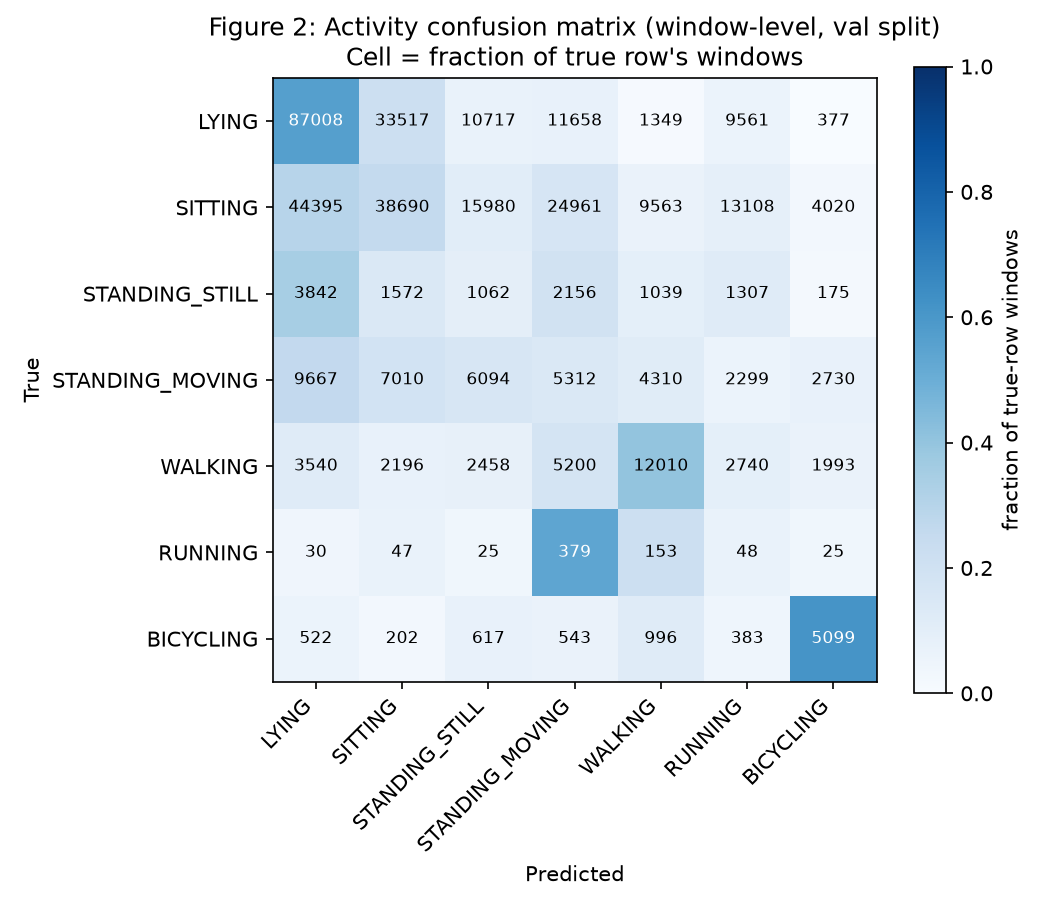
\includegraphics[width=0.55\linewidth]{fig2_confusion_matrix.png}
\caption{\textbf{Confusion matrix} on held-out users (rows true, columns predicted). F1 per activity: lying 0.63, sitting 0.29, standing in place 0.06, standing and moving 0.14, walking 0.45, running 0.01, bicycling 0.45.}
\label{fig:fig2}
\end{figure}

\paragraph{Evidence.} With the model's labels, 41\% of evidence answers overlap the truth by at least half (Figure~\ref{fig:fig3}). The evidence is often partly right: 71\% is accepted if only 10\% overlap is required.

\begin{figure}[h]
\centering
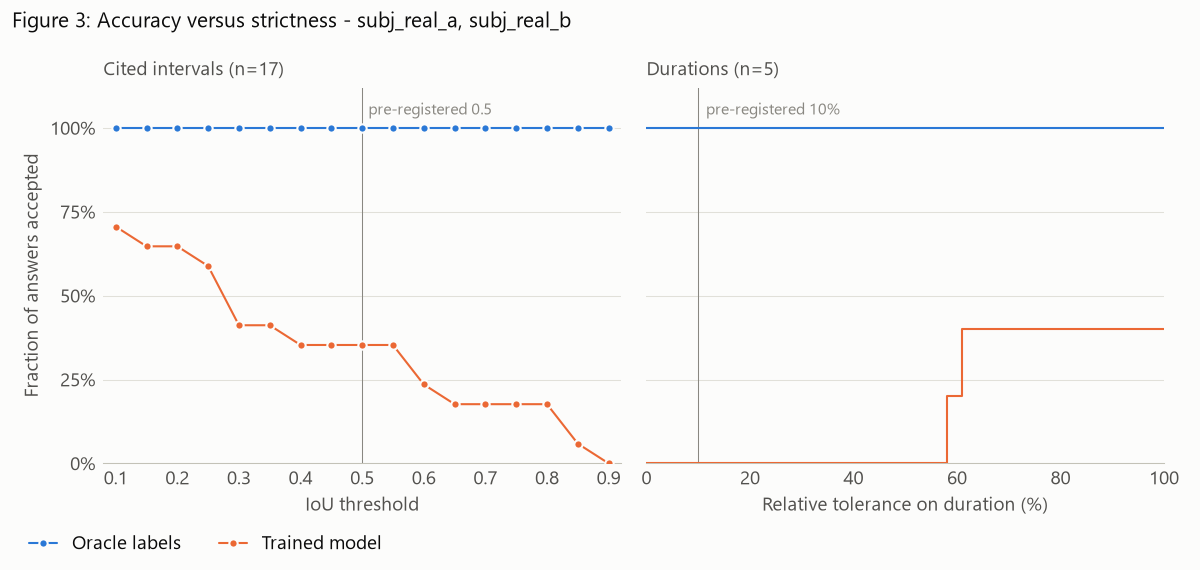
\includegraphics[width=0.85\linewidth]{fig3_accuracy_vs_strictness.png}
\caption{\textbf{Accuracy versus strictness.} Left: share of the 17 evidence answers accepted as the required overlap rises. Right: share of the 5 duration answers within each error margin; with the model's labels, none is within 55\%.}
\label{fig:fig3}
\end{figure}

\paragraph{Open-ended questions.} Of 16 questions about behaviours outside the seven activities, 6 were answered from the signal (such as fidgeting, sleep and exercise), 9 got an honest ``cannot tell'', and 1 (``did she go for a jog?'') was read as running. The judge rated the 46 open-ended explanations \textbf{4.45 out of 5} on average: 4.41 for citing real measurements, 4.63 for supporting the answer, and 4.29 for plausibility. Its two independent runs agreed closely (weighted $\kappa$ between 0.76 and 0.87). Its lowest scores went to two answer templates we could improve: ``mostly at rest or active?'' cites no measurement, and the cycling answer does not explain its durations.

% ---------------------------------------------------------------------
\section{Efficiency}
\label{sec:efficiency}
All costs were measured on a laptop CPU (AMD Ryzen 7 4800H, 8\,GB RAM). The energy figure is estimated from the processor's rated power, since we had no power meter.

\begin{table}[h]
\centering\small
\begin{tabular}{@{}lr@{}}
\toprule
Model size & 9,975 parameters, 0.047\,MB \\
Time per window (median) & 0.40\,ms \\
Energy per window (estimate) & 7.6\,mJ \\
Time to answer one question (median) & 67\,ms \\
Peak memory, answering & 299\,MB \\
\bottomrule
\end{tabular}
\caption{Resource cost.}
\label{tab:cost}
\end{table}

\paragraph{Compression.} We made three smaller models without retraining: one storing weights as 8-bit integers, and two with 30\% and 60\% of the network's filters removed (Figure~\ref{fig:fig4}). The 8-bit model is 27\% smaller with no loss in accuracy. It even scored slightly higher, but on 34 questions that is noise. Removing filters shrinks the model further, at a growing cost in accuracy. All versions run in about the same time, so at this size compression saves space, not time.

\begin{figure}[h]
\centering
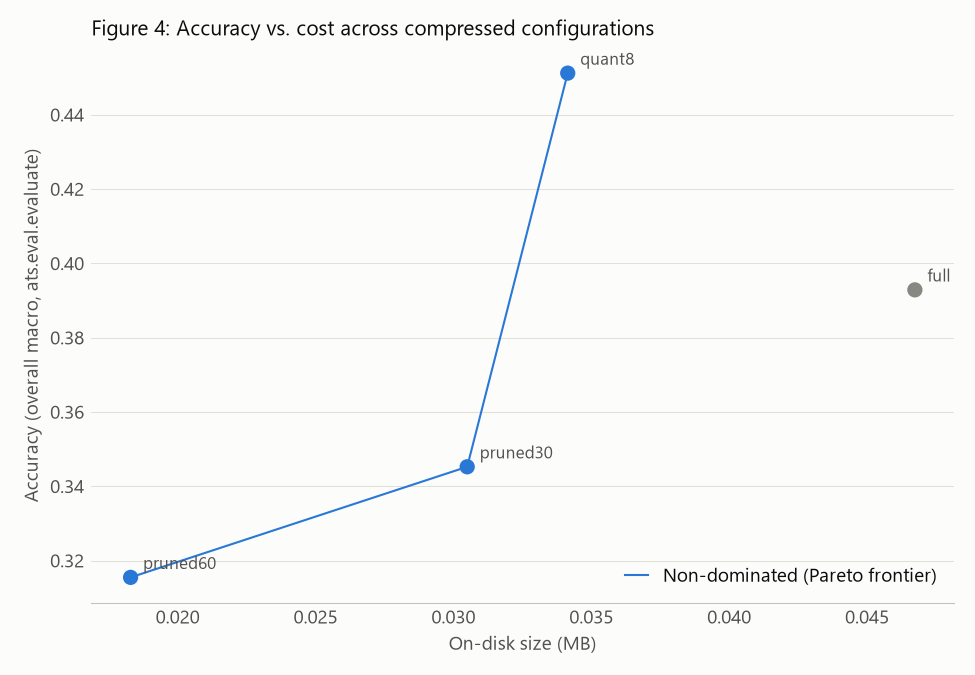
\includegraphics[width=0.62\linewidth]{fig4_pareto.png}
\caption{\textbf{Accuracy versus model size.} The line joins the versions that no other version beats on both.}
\label{fig:fig4}
\end{figure}

\paragraph{Robustness.} Dropping up to half of the raw samples costs little accuracy (0.393 to 0.375), and 70\% only brings it to 0.357 (Figure~\ref{fig:fig5}).

\begin{figure}[h]
\centering
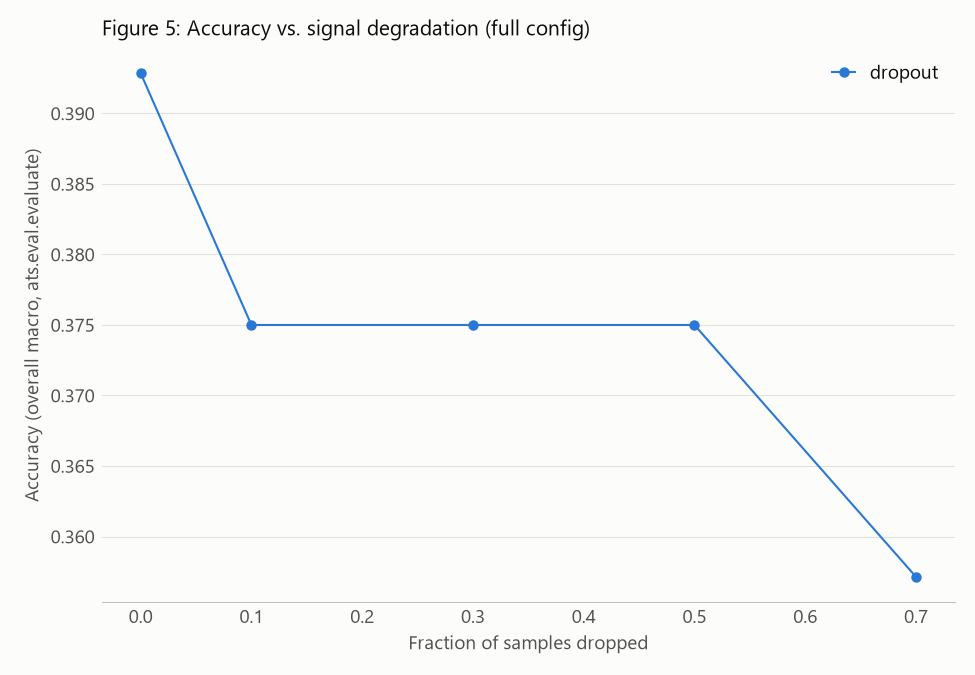
\includegraphics[width=0.62\linewidth]{fig5_robustness.png}
\caption{\textbf{Robustness}: accuracy as more of the raw signal is dropped.}
\label{fig:fig5}
\end{figure}

% ---------------------------------------------------------------------
\section{Limitations}
\begin{itemize}
  \item \textbf{Recognition is the bottleneck.} The answering made no errors, but the model's labels limit the system to 15 of 34 on real users.
  \item \textbf{Small test sets.} We wrote our own questions, and the two real users were in the training group, so the real-user numbers are likely optimistic.
  \item \textbf{Stillness is our only measured signal property,} so other behaviours rely on labels or get ``cannot tell''.
  \item \textbf{Long evidence lists.} On multi-day recordings an answer can cite over a hundred intervals, which is correct but hard to read.
\end{itemize}

% ---------------------------------------------------------------------
\section{Contributions}
\textbf{Abhinav Kumar Singh (22CS30005)} built the signal side: data download and cleaning, resampling, windowing, training the recognition model (Figure~\ref{fig:fig2}), cost measurement, compression and robustness testing (Figures~\ref{fig:fig4} and~\ref{fig:fig5}).

\noindent\textbf{Harsh Chattar (22CS30028)} built the answering side: the timeline, question matching, the operations behind every answer, the answers for open-ended questions and the checker. He also built the evaluation: the test questions, scoring and explanation rating (Figures~\ref{fig:fig1} and~\ref{fig:fig3}).
\begin{thebibliography}{9}\small
\bibitem{extrasensory} Y.~Vaizman, K.~Ellis, G.~Lanckriet. Recognizing detailed human context in-the-wild from smartphones and smartwatches. \emph{IEEE Pervasive Computing}, 2017. \url{http://extrasensory.ucsd.edu/}
\bibitem{torch} A.~Paszke et al. PyTorch: an imperative style, high-performance deep learning library. NeurIPS, 2019.
\bibitem{qwen} Qwen Team. Qwen2.5 technical report. arXiv:2412.15115, 2024.
\bibitem{claude} Anthropic. Claude Haiku 4.5, accessed through OpenRouter (\url{https://openrouter.ai/}).
\end{thebibliography}

\end{document}
